\documentclass{article}
\usepackage[margin=1in]{geometry}
\usepackage{graphicx,hyperref}
\title{CSCI 202, Spring 2017, Lab \# 2}
\author{Geoffrey Matthews}

\begin{document}
\maketitle

\begin{description}

\item[Due date:] Midnight, Monday, April 24.

\item[Goals:] Adding a bit of CSS style to some HTML.

\item[Zip your folder:]

  Put all your files (including the supporting files) in a single
  folder and  make a compressed (zip) archive of the folder.

\item[Style files:]  You will not create any style files for this
  assignment.  All styling will be done with an internal style sheet
  for each file, marked off with the \verb|<style>| tag.

  This will make it easier for the grader to see both your html and
  your css at once.

\item[Files:]  You will create the following {\tt .html} files.
    All pages should pass the W3C validator with no errors.

    \item[index.html]     The title and {\tt h1} header of this page
      will be {\bf CSCI 202, Lab 2}

      This page will have an unordered list of links to the other
      pages of the lab.

      The background and text colors
      of this page will be colors of your choice (not black and white,
      but a good legible combination).

  \item[page01.html]


    The title and {\tt h1} header of this page will be {\bf Web
      Images}.

    Copy the files \verb|web_images.html| and \verb|cubes.gif| found
    on the github repository to your own computer and put them in the
    same folder as your html files.
    
  Use the cubes image to make a background image running down the left
  side of your page.  Use the background and margin properties to
  indent the text to the right of the background image.  Your final
  page should look something like this:

  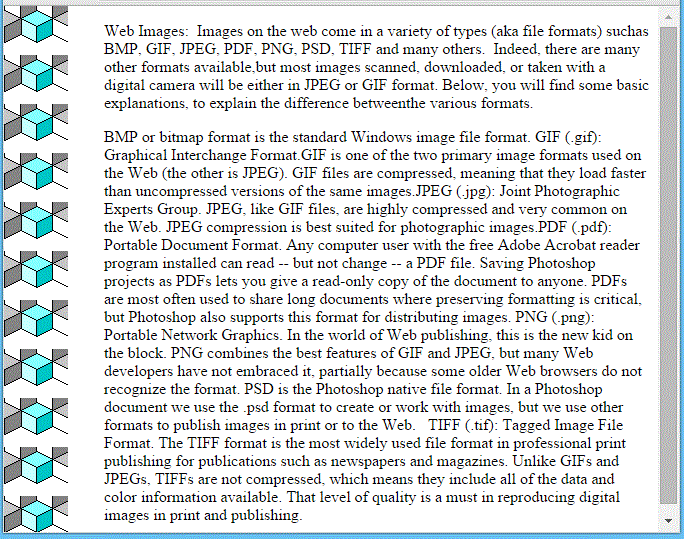
\includegraphics[scale=0.5]{page.png}

\item[page02.html]
  The title and {\tt h1} header of this page will be {\bf Generic Font
    Families}. 

  Look up the names of the five generic font families found here:
  \url{https://www.w3.org/Style/Examples/007/fonts.en.html}.

  Display a list on this page of each of the names for the generic
  font families, each typeset with its own generic font family.  For
  example, assuming that ``Fubar'' is a generic font family, the word
  ``Fubar'' would be displayed in the ``Fubar'' typeface.

\item[page03.html]

    The title and {\tt h1} header of this page will be
  {\bf Sick}.

  The poem for this page is on the github repository in the file named
  {\tt sick.txt}.  Style this page so that each stanza of the poem is
  a paragraph with an enlarged first letter in a different color (your
  choice).  The {\tt h1} header should also be in the same color.

  Also include a box that floats to the left of the text with your
  name, the class number, and ``Lab 2''.  The final result should look
  something like this:

  {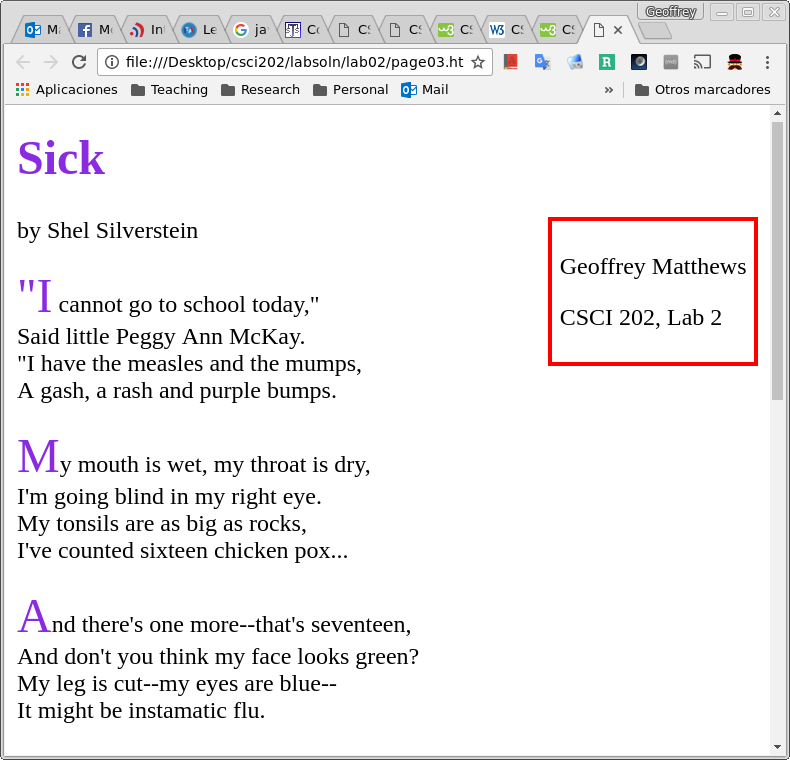
\includegraphics[scale=0.5]{sick.png}}




\end{description}

\end{document}
